\documentclass[aps,prl,twocolumn,showpacs,superscriptaddress,floatfix]{revtex4-1}
%groupedaddress,
\addtolength{\abovecaptionskip}{-0.1in}
\addtolength{\belowcaptionskip}{-0.2in}

\usepackage[utf8]{inputenc} %useful to type directly diacritic characters
\usepackage{amssymb,amsmath}
\usepackage{graphicx}
\usepackage{braket}
\usepackage{siunitx}
\usepackage{xcolor}
\usepackage{physics}

% MACROS
% AMO abbreviations
\def\lambdar{\lambda_{\rm R}}                           % raman lambda
\def\lambdal{\lambda_L}                            		% lattice lambda
\def\kr{k_{\rm R}}                            			% kr
\def\kl{k_L}                            				% kL
\def\Er{E_{\rm R}}                            			% kr
\def\El{E_L}                            				% kL
\def\Rb87{^{87}\mathrm{Rb}}                             % Rb 87
\def\K40{^{40}\mathrm{K}}                    		    % K 40 

\def\ex{\mathbf{e}_x}  
\def\ey{\mathbf{e}_y}  
\def\ez{\mathbf{e}_z}  

\begin{document}

%Title of paper
\title{We have learned things}
\author{F.~Author}
\author{S.~Author}
\author{I.~B.~Spielman}
\affiliation{Joint Quantum Institute, National Institute of Standards and Technology, and University of Maryland, Gaithersburg, Maryland, 20899, USA}
\email{spielman@nist.gov}
\date{\today}

\begin{abstract}
This was really exciting
\end{abstract}

\maketitle

%----------------------------------------------------------------------------------------
%	 Introduction
%----------------------------------------------------------------------------------------

We introduce neat things that might relate to Ian's thesis~\cite{Spielman2004}.

%----------------------------------------------------------------------------------------
%	Fig1
%----------------------------------------------------------------------------------------

\begin{figure}[t]
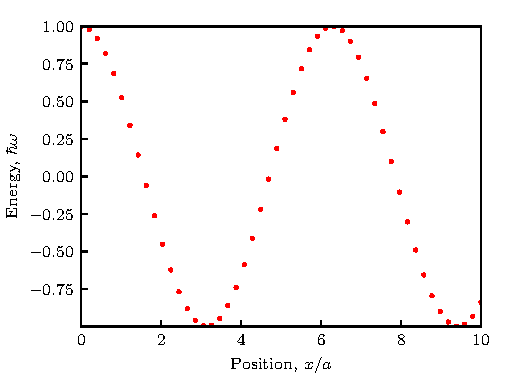
\includegraphics{Fig_Setup.pdf}
\caption{We have discovered sinusoidal oscillations of energy as a function of position.}
\label{Fig_Setup}
\end{figure}

%----------------------------------------------------------------------------------------

%----------------------------------------------------------------------------------------
%	 Discussion and Outlook
%----------------------------------------------------------------------------------------

%----------------------------------------------------------------------------------------
%	 Acknowledgements
%----------------------------------------------------------------------------------------
\begin{acknowledgments}
The authors thank ABC for productive discussions, and DEF and GHI for carefully reading the manuscript.
This work was partially supported by the National Institute of Standards and Technology, and the National Science Foundation through the Quantum Leap Challenge Institute for Robust Quantum Simulation (grant OMA-2120757).
\end{acknowledgments} 

\bibliography{main}

\end{document}